\section*{Cycle 2 Experiment 1 }

\section{\Large{Socket Programming: TCP}}

\subsection{Aim}
\large To implement Client-Server communication using Socket Programming and TCP as transport
layer protocol.

\subsection{Theory}
TCP (Transmission Control Protocol) is one of the main protocols in TCP/IP networks. Transmission control protocol (TCP) is a network communication protocol designed to send data packets over the Internet. TCP is a transport layer protocol in the OSI layer and is used to create a connection between remote computers by transporting and ensuring the delivery of messages over supporting networks and the Internet.\\

It is a connection-oriented protocol, which means that a connection is established and maintained until the application programs at each end have finished exchanging messages.\\
\\
TCP programs are implemented in two parts:\\

• Server: A server program listens for a connection. On getting a request, the server accepts a connection. After the connection is established, server and client can exchange messages.\\

• Client: A client program requests some service. A client program request for some resources to the server and server responds to that request. Client initiates the connection establishment. The server accepts connection and
client can request services by exchanging messages.\\
\\
\textbf{Sockets}\\
Implementation of the above two programs (Client and Server) is to be done with the help of sockets. A socket is one endpoint of a two-way communication link between two programs running on the network. Client program and server program
create and use sockets to communicate with each other.

\subsection{Algorithm}
\begin{verbatim}
Algorithm for the client

1 START
2 Create the socket using the function socket()
3 Configure socket details
4 Connect the socket to the server using function connect()
5 Receive the message from the server using recv()
6 Print the received message
7 STOP


Algorithm for the Server

1 START
2 Configure socket details
3 Set all bits of the padding field to 0 using memset ()
4 Bind the address struct to the socket using bind ()
5 Listen to the socket
6 A new socket for the incoming connections created using accept()
7 Send message to the incoming connection using send()
8 STOP
\end{verbatim}

\subsection{Program \& Output}
\begin{verbatim}
//Socket Programming:TCP
//Server Side

#include<stdio.h>
#include<sys/socket.h>
#include<netinet/in.h>
#include<string.h>

int main(){
    int welcomeSocket, newSocket;
    char buffer[1024];
    struct sockaddr_in serverAddr;
    socklen_t addr_size;
    struct sockaddr_storage serverStorage;

    welcomeSocket = socket(PF_INET, SOCK_STREAM, 0);
    serverAddr.sin_family = AF_INET;
    serverAddr.sin_port = htons(7891);
    serverAddr.sin_addr.s_addr = inet_addr("127.0.0.1");
    memset(serverAddr.sin_zero, '\0', sizeof serverAddr.sin_zero);

    bind(welcomeSocket, (struct sockaddr*)&serverAddr, sizeof(serverAddr));

    if (listen(welcomeSocket, 5 ) == 0)
        printf("Listening for the client to be live..\n");
    else
        printf("Error\n");

    addr_size = sizeof serverStorage;
    newSocket = accept(welcomeSocket, 
                (struct sockaddr*)&serverStorage, &addr_size);

    strcpy(buffer, "Hello World\n");
    send(newSocket, buffer, 13, 0);

    return 0;
}


//Client Side

#include<stdio.h>
#include<sys/socket.h>
#include<netinet/in.h>
#include<string.h>

int main(){
    int clientSocket;
    char buffer[1024];
    struct sockaddr_in serverAddr;
    socklen_t addr_size;

    //Create socket
    clientSocket = socket(PF_INET, SOCK_STREAM, 0);

    serverAddr.sin_family = AF_INET;
    serverAddr.sin_port = htons(7891);
    serverAddr.sin_addr.s_addr = inet_addr("127.0.0.1");
    memset(serverAddr.sin_zero, '\0', sizeof serverAddr.sin_zero);
    addr_size = sizeof serverAddr;
    connect(clientSocket, (struct sockaddr*)&serverAddr, addr_size);
    recv(clientSocket, buffer, 1024, 0);
    printf("Data received = %s", buffer);

    return 0;
}
\end{verbatim}
\begin{figure}[h]
            \centering
            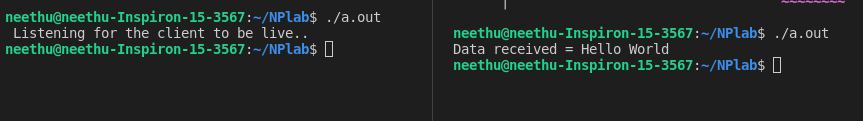
\includegraphics[scale=0.55]{img/e7.png}
\end{figure}

\subsection{Result}
Implemented the program for the Client-Server communication using Socket Programming and TCP as transport layer protocol using C language in Ubuntu 18.04 with kernel and the above outputs were obtained.

